%
% The first command in your LaTeX source must be the \documentclass command.
\documentclass[sigconf, review, anonymous]{acmart}

\usepackage{balance}
\usepackage[norelsize,ruled,linesnumbered,lined,commentsnumbered]{algorithm2e}

%
% \BibTeX command to typeset BibTeX logo in the docs
\AtBeginDocument{%
  \providecommand\BibTeX{{%
    \normalfont B\kern-0.5em{\scshape i\kern-0.25em b}\kern-0.8em\TeX}}}

\SetKwRepeat{Do}{do}{while}

\begin{document}

\title{StreamNet: Enabling Large Scale DAG based Nakamoto Consensus through Streaming Graph Computing}

%TRIAS StreamNet is a DAG (Directed Asyclyc Graph) blockchain design rooted from the existing mature systems. 
Considering major issues in the existing DAG systems such as centralization caused by the introduction of Coordinator, double-spending and sybil attacks, slow transaction speed etc. 
We designed and implemented the StreamNet system which is forked from the IOTA implementation.
By leveraging the Topological sorting and Katz centrality computation, we infer a pivotal chain along the path of each topological level in the graph,
and each block in the pivotal chain will have the highest Katz centrality score, which could be used as the entry point for the tip selection algorithm.
In addtion, with comprehensive integration of information such as transaction (vertices), 
transaction approval information (edges), and network structure (such as community structure) we designed the tip selection algorithm that obeys the local modifier method and can detect and avoid double spend / sybil attacks.


\maketitle

%
% The abstract is a short summary of the work to be presented in the article.

\keywords{Block chain, DAG }

\section{Introduction}
Ever since bitcoin \cite{nakamoto2008bitcoin} has been proposed, blockchain technology has been widely studied for $10$ years. 
Extensive adoptions of blockchain technologies was seen in real world applications such as 
financial services with potential regulation challenges \cite{michael2018blockchain, tapscott2017blockchain}, 
supply chains \cite{korpela2017digital,tian2016agri, abeyratne2016blockchain}, 
health cares \cite{azaria2016medrec,yue2016healthcare} and IOT devices \cite{christidis2016blockchains}.
The core of blockchain technology depends on the consensus algorihtms applying to the open distrubuted computing world.
Where computers can join and leave the network and these copmuters can cheat.

As the first protocol that can solve the so called Byzantine general's problem, 
bitcoin system suffers from the problem of low transaction rate with a transaction per second (TPS) of approximately $7$, and long confirmation time (about an hour).
As more and more machines joined the network, they are competing for the privileges to attach the block (miners) which result in huge waste of electric power.
While sky rocketing fees are payed to make sure the transfers of money will be placed in the chain.
On par, there are multiple proposals to solve the low transaction speed issue. 

One method intends to solve the speed problem without changing the chain data structure, for instance, 
the bitcoin cash (BCH) fork of bitcoin (BTC) system tries to improve the throughput of the system by enlarging the data size of each block from $1$ Mb to $4$ Mb. 
To minimize the cost of POW, a proof of stake method POS \cite{wood2014ethereum} is proposed to make sure that only those who in the network have the privilege to attach the block only if they have a large amount of token shares.
Anohter idea targeting at utilizing the power in POW to do useful and meaningful tasks such as training machine learning models are also proposed \cite{matthew2017aion}.
In addition, inspired by the PBFT algorithm \cite{castro1999practical} and a set of its relateted variations, so called hybrid (or consortium) chain was proposed. 
The general idea is to use two step algorithm, the first step is to elect a commiette, the second step is collecting committee power to employ PBFT for consensus.
Bitcoin-NG \cite{eyal2016bitcoin} is the early adoptor of this idea, which splits the blocks of bitcoin into two groups, one is for master election and another for regular transaction blocks. 
Honey-badger \cite{miller2016honey} is the system that firstly introducted the consensus commitee, it uses a predefined memebers to perform PBFT algorithm to reach consensus.  
The Byzcoin system \cite{kogias2016enhancing} brought forth the idea of POW for the commitee election, and uses a variation of PBFT called collective signing for speed purposes.
The Algorand \cite{gilad2017algorand} utilizes a random function to anonymously elect commetee and use this commitee to commit blocks, and the member of the commitee only have one chance to commit block.
All these systems have one common feature, the split of layers of players in the network, which results in the complexity of the implementation of the system.

While aforemetioned methods are trying to avoid side chains, another thread of effort is put on using direct acyclic graph DAG to merge side chains.
The first ever idea comes with growing the blockchain with trees instead of chains \cite{sompolinsky2013accelerating}, which results in the well known GHOST protocol \cite{sompolinsky2015secure}.
If one block links to $\geq 2$ previous blocks, then the data structure grows like a DAG instead of tree \cite{sompolinsky2016spectre, sompolinskyphantom, lewenberg2015inclusive}.
There is a improvement of the GHOST based DAG algorithm which can achieve $6000$ of TPS in reality \cite{li2018scaling}.
Another set of methods tried to avoid finality of constructing a linear total order by introducing the probability of confirmation in the network \cite{popov2016tangle, churyumov2016byteball}. 
However, suffering from engineering issues, mainly due to the lack of transaction frquency and the growing complexity due to the network expansion.
These system in reality are rely on centralized mehods to maintain their stability.
Some of the side chain methods also borrows the idea of DAG, such as nano \cite{lemahieu2018nano} and vite \cite{liuvite}.

Social network analysis has widely adopted the method of streaming graph computing \cite{ediger2011tracking, green2012fast, ediger2012stinger} which deals
with how to quickly maintain information on a temporally or spatially changing graph without traversing the whole graph. 
We view the DAG based method as a streaming graph problem which is about how to compute the total order and achieve consensus without consuming more computing power.
In distributed database systems, the problem of replicating data across machines is a well studied topic \cite{demers1988epidemic}.
Due to the low efficiency of the bitcoin network, there are multiple ways to accelerate the message passing efficiency \cite{klarmanbloxroute}, however, they did not deal with the network complexity. 
We view the problem of scaling DAG system in the network of growing size and topological complexity as another challenging issue, and proposed our own gossip solution.
The main contribution of this paper is how to utilize the streaming graph analysis methods and new gossip protocol to bring the DAG systems into real decentralized, and stabilized growing system.

\section{Basic concepts}
\subsection{Basic data structure}
StreamNet is a Directed Acyclic Graph, where each vertex in the $DAG$ represents a block and the directed edge represents a confirmation relationship between blocks.
For instance, vertex $0$ in Figure~\ref{simple_sn} represents the Genesis block, which is by default a confirmed block.
Vertex $1$, on the other hand, represents the first block, which is confirmed by the subsequent block $2$, $3$ and $4$. 
When a new block is not confirmed, it is called a tip. For example, in Figure~\ref{simple_sn}, block $6$ is a tip.

\begin{figure}[!ht]
\begin{center}
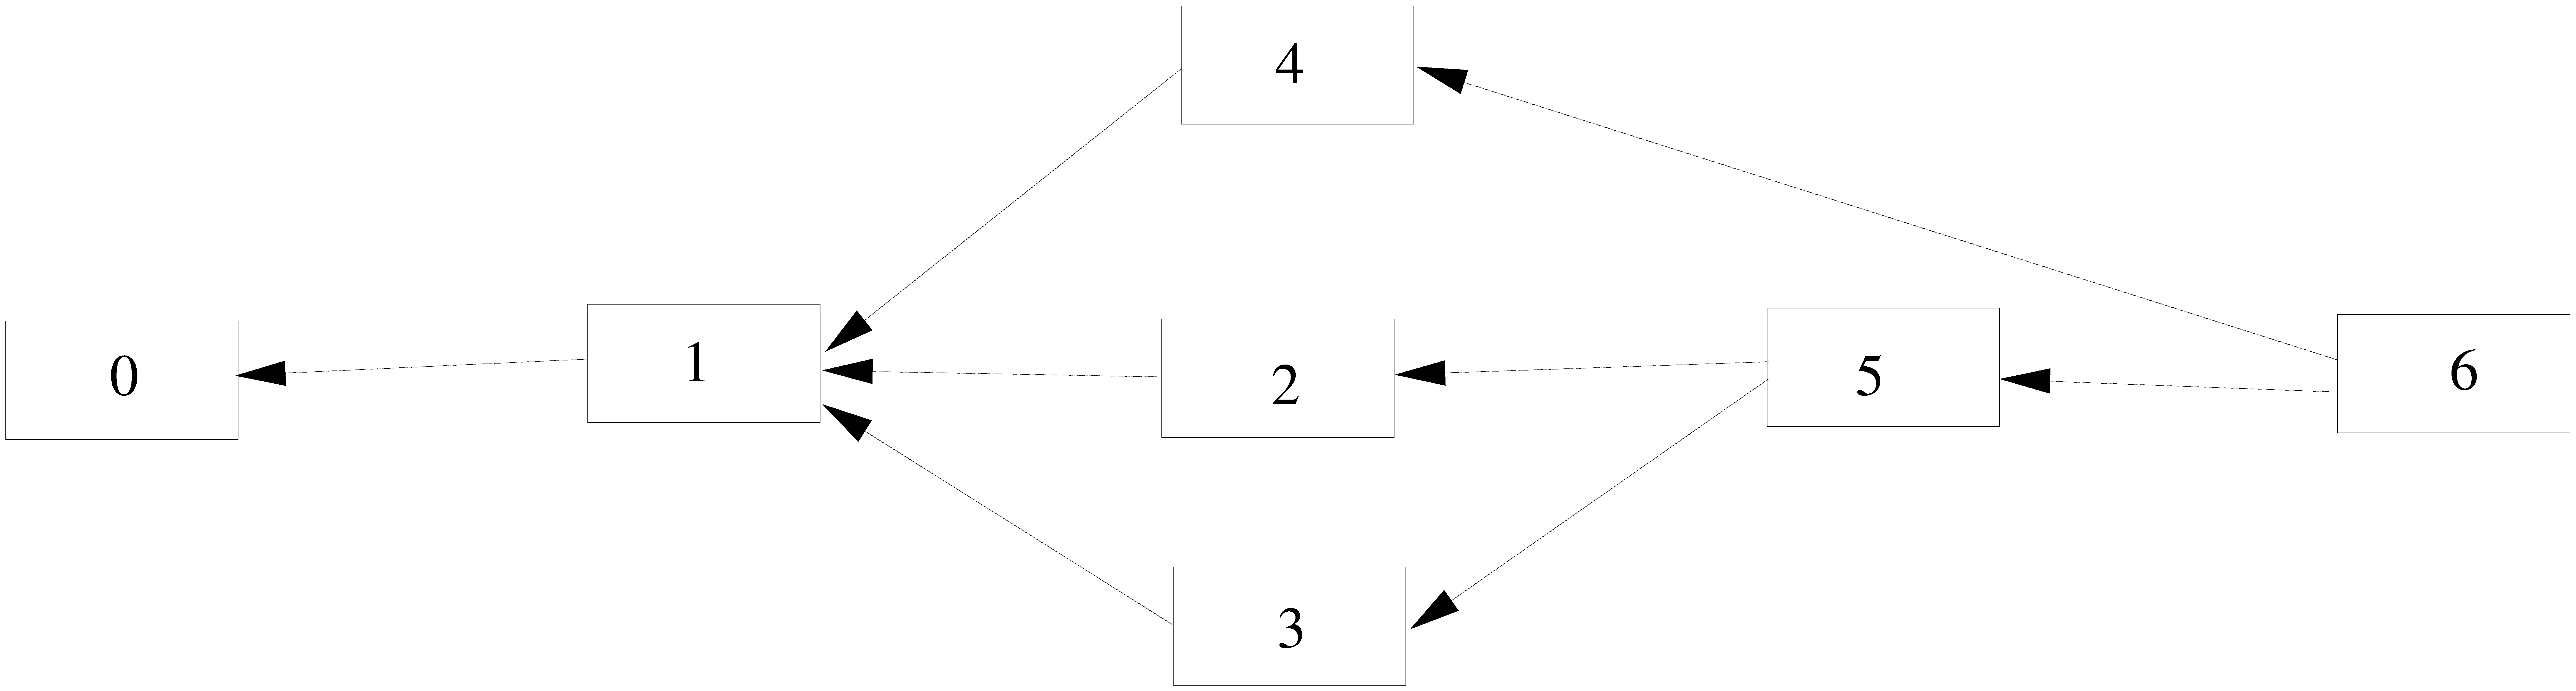
\includegraphics[width=0.45\textwidth]{figures/simple_sn.eps}
    \caption{
        Example of the StreamNet data structure.
     }
\label{simple_sn}
\end{center}
\end{figure}



\subsection{Transaction}
\subsubsection{Genesis transaction}

\begin{figure}[!ht]
\begin{center}
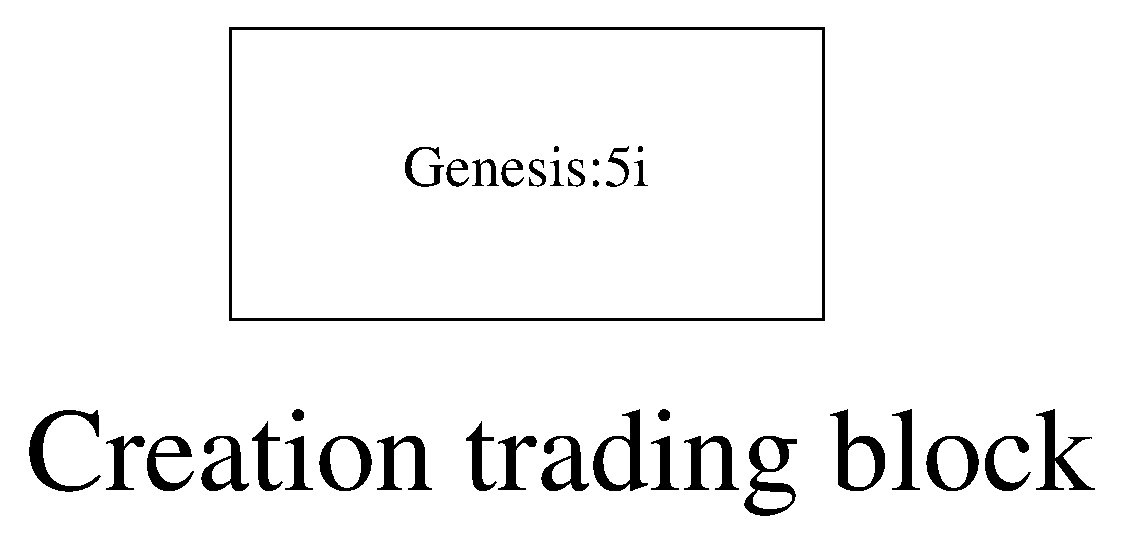
\includegraphics[width=0.15\textwidth]{figures/genesis.eps}
    \caption{
        The creation of genesis node.
     }
\label{genesis}
\end{center}
\end{figure}

There is no concept of mining in StreamNet, and all tokens are included in the Genesis Node.
In Figure~\ref{genesis}, an initial transaction is created with $5$ tokens.


\subsubsection{Transaction Content}

\begin{figure}[!ht]
\begin{center}
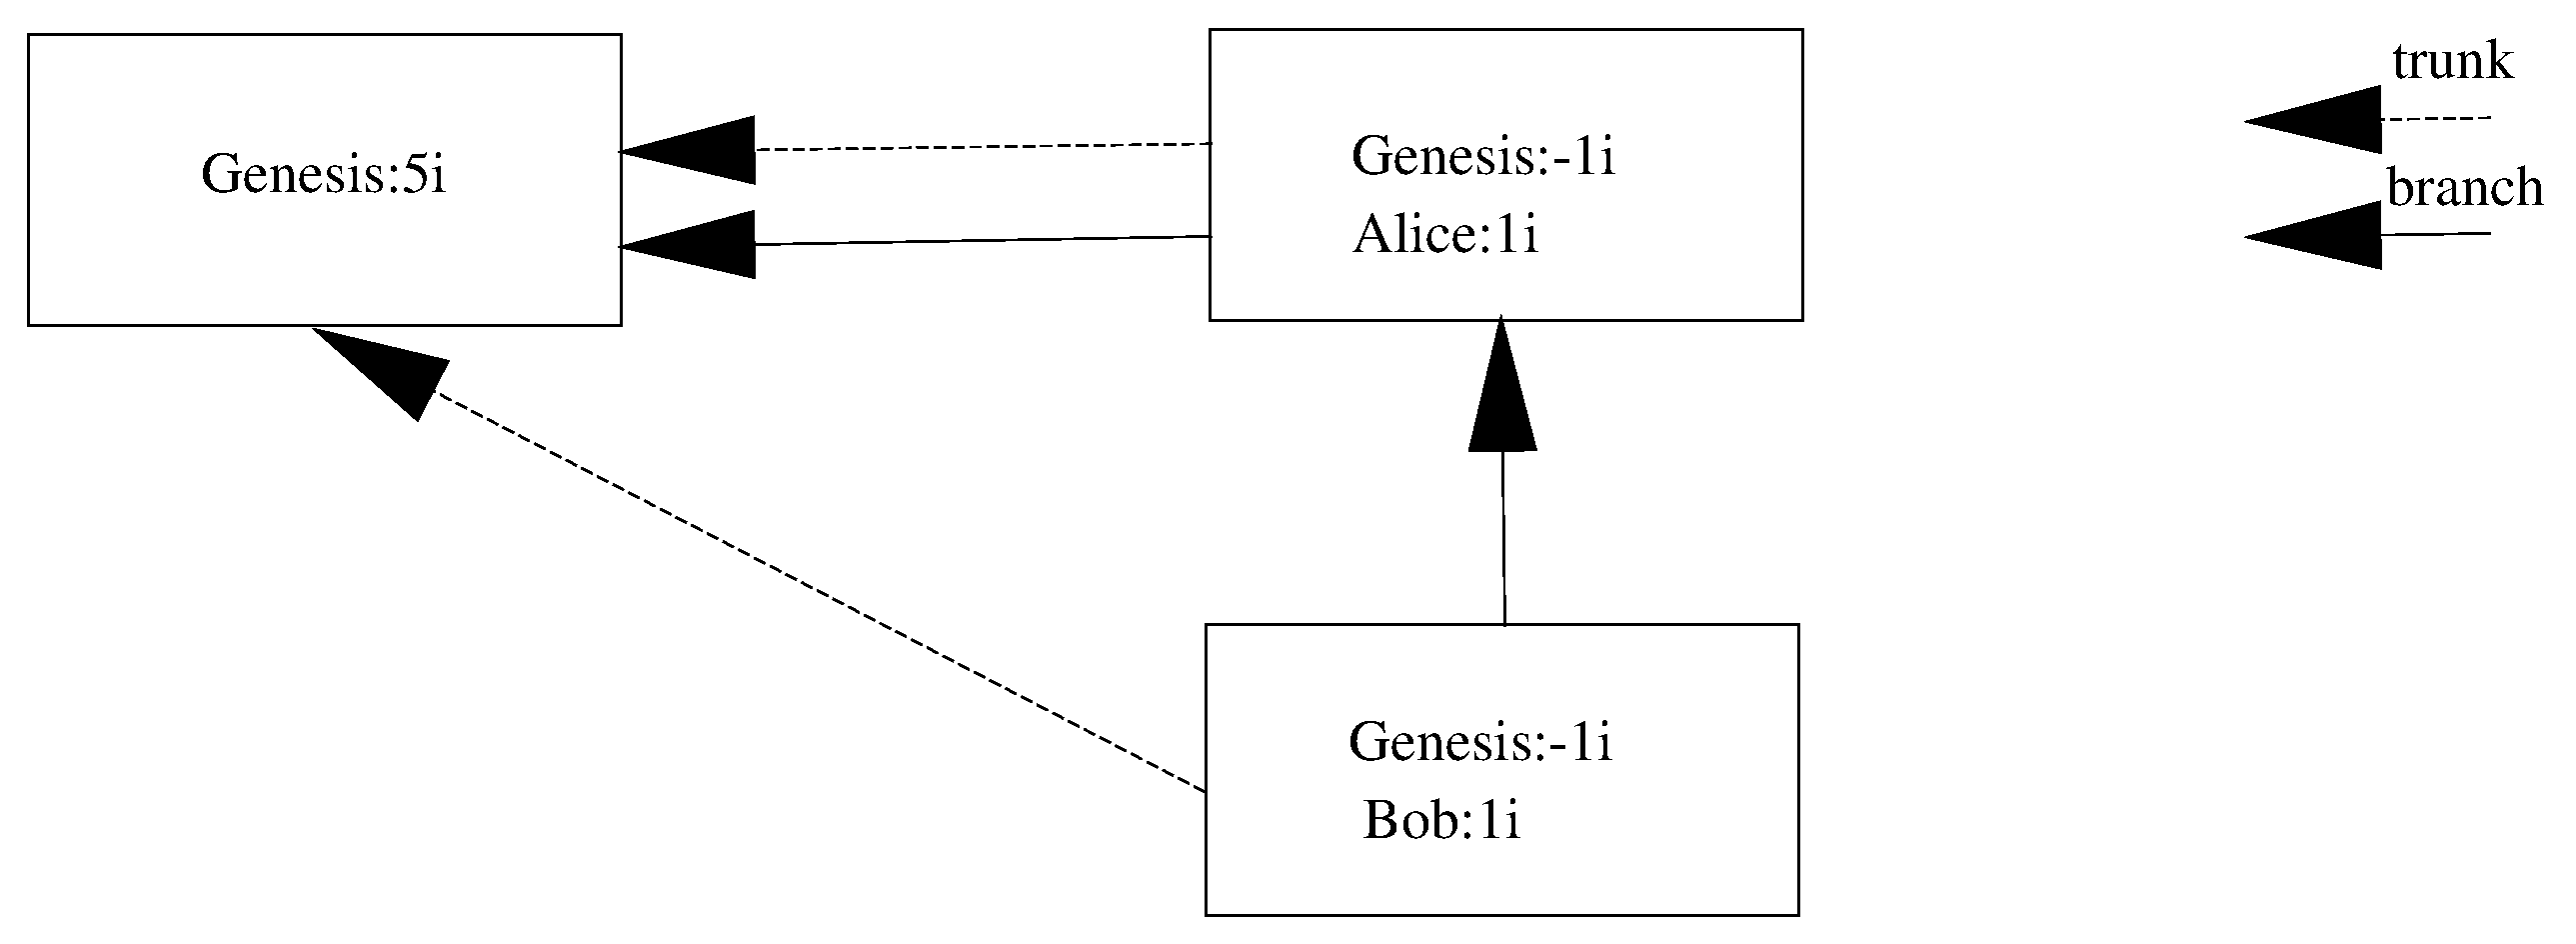
\includegraphics[width=0.35\textwidth]{figures/simple_transfer.eps}
    \caption{
        An example of token transfers.
     }
\label{simple_transfer}
\end{center}
\end{figure}

Assume that in Figure~\ref{genesis}, Genesis wants to transfer $1$ token to Alice, 
and then hopes to transfer $1$ token to Bob and attach the transaction node to StreamNet, the resulting $DAG$ is shown in Figure~\ref{simple_transfer}.
Here, each transaction must find two tip transactions to confirm, namely trunk and branch transactions.
For example, the Genesis $\rightarrow$ Alice transaction confirms the Genesis transaction itself,
while the Genesis $\rightarrow$ Bob transaction confirms the Genesis transaction and the Genesis $\rightarrow$ Alice transaction.
When a transaction wants to be attached to StreamNet, it must do enough Proof of Work (POW),
but this POW differs from Bitcoin in that its difficulty is fixed and therefore does not need the participation of miners.

\subsubsection{Transaction validation (approve)}

\begin{figure}[!ht]
\begin{center}
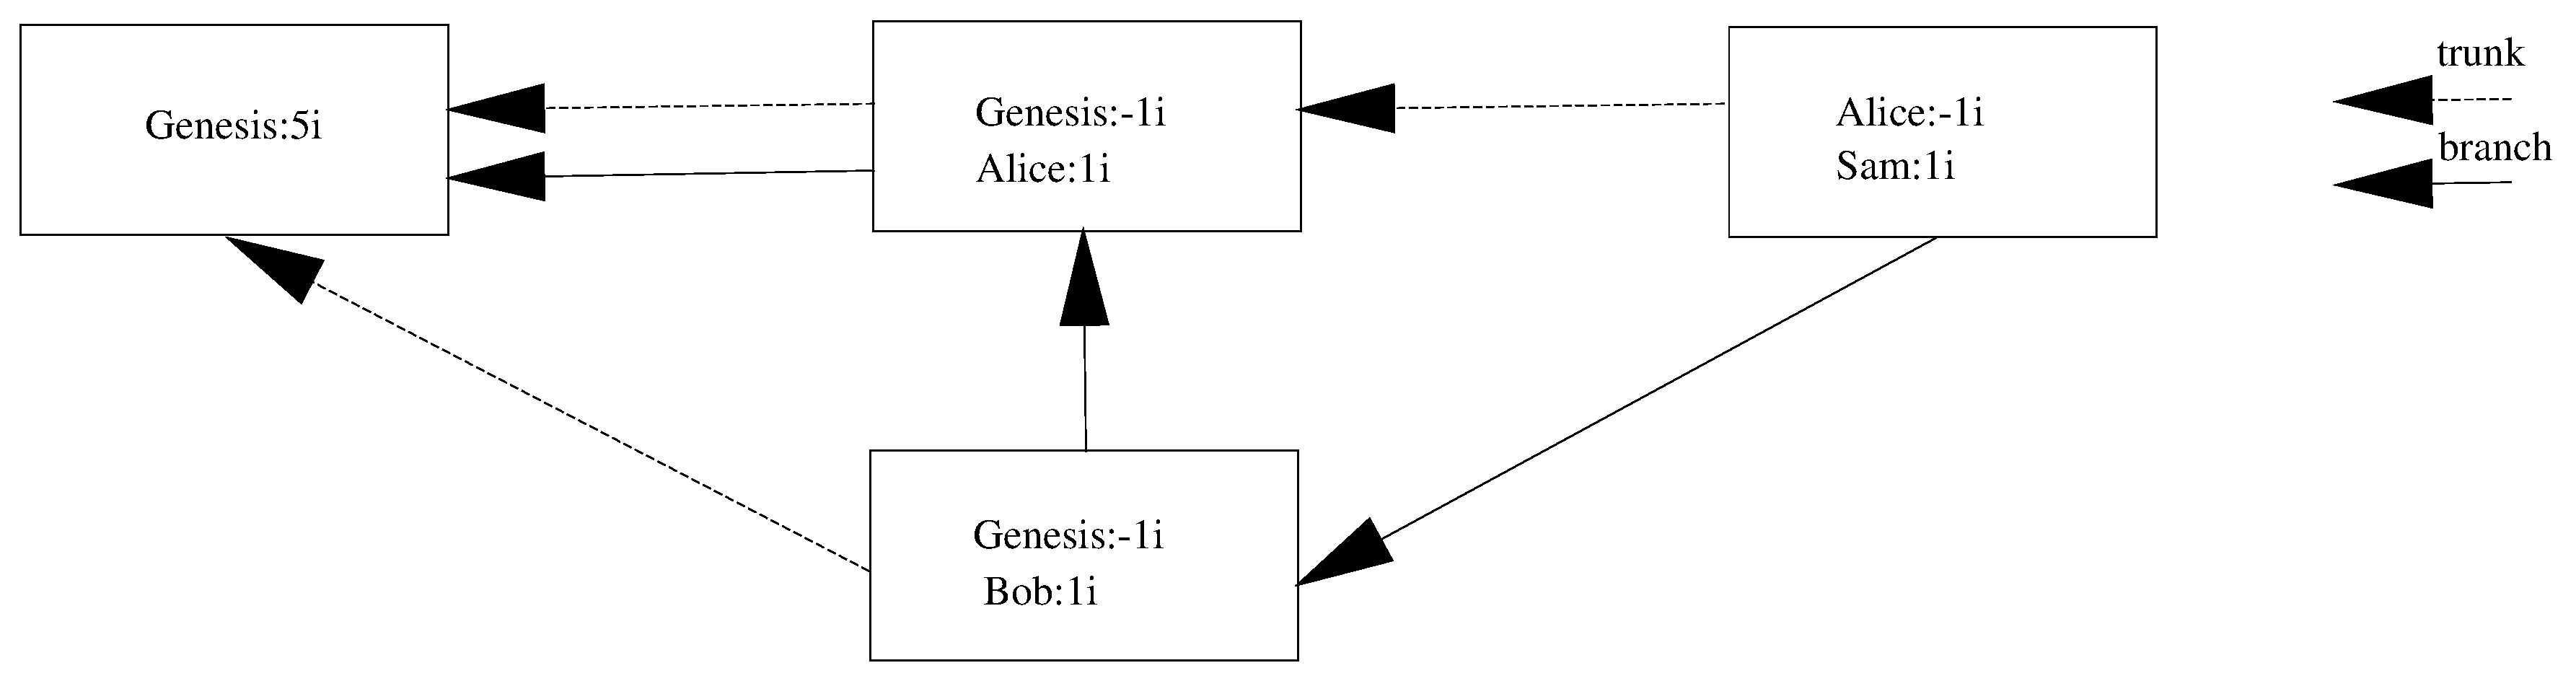
\includegraphics[width=0.35\textwidth]{figures/txn_success.eps}
    \caption{
        An example of succesfull token transfer.
     }
\label{txn_success}
\end{center}
\end{figure}

Because a new transaction needs to find two tip transactions to approve, the validation process is diveded into two steps:

\begin{itemize}
\item Start from Genesis, verify all transactions that are directly or indirectly referenced, 
mainly to see if this will result in a negative balance or loss of the token \cite{gal_2018}.
For example, in Figure~\ref{txn_success}, the Alice $\rightarrow$ Sam transfer needs to validate transactions it indirectly or directly approves.
It constructs a topological transfer sequence, 
namely (Genesis) $\rightarrow$ (Genesis $\rightarrow$ Alice) $\rightarrow$ (Genesis $\rightarrow$ Bob) $\rightarrow$ (Alice $\rightarrow$ Sam),
and find that each step does not violate the principle of transfer, which means the verification is successful.
In Figure~\ref{txn_fail}, the same topology sequence, when verifying (Genesis $\rightarrow$ Bob), 
because the Genesis balance will be reduced to -1, the verification fails.
As an honest node, Alice $\rightarrow$ Sam transaction Will find a new tip to verify,
but it can also choose to cheat, attach this transaction to the selected tip.
However, it is likely to result in subsequent rejection of this transaction.
\item At the mean time, the signature of the transaction needs to be checked to ensure that the link relationship has not been tampered with.
\end{itemize}

\begin{figure}[!ht]
\begin{center}
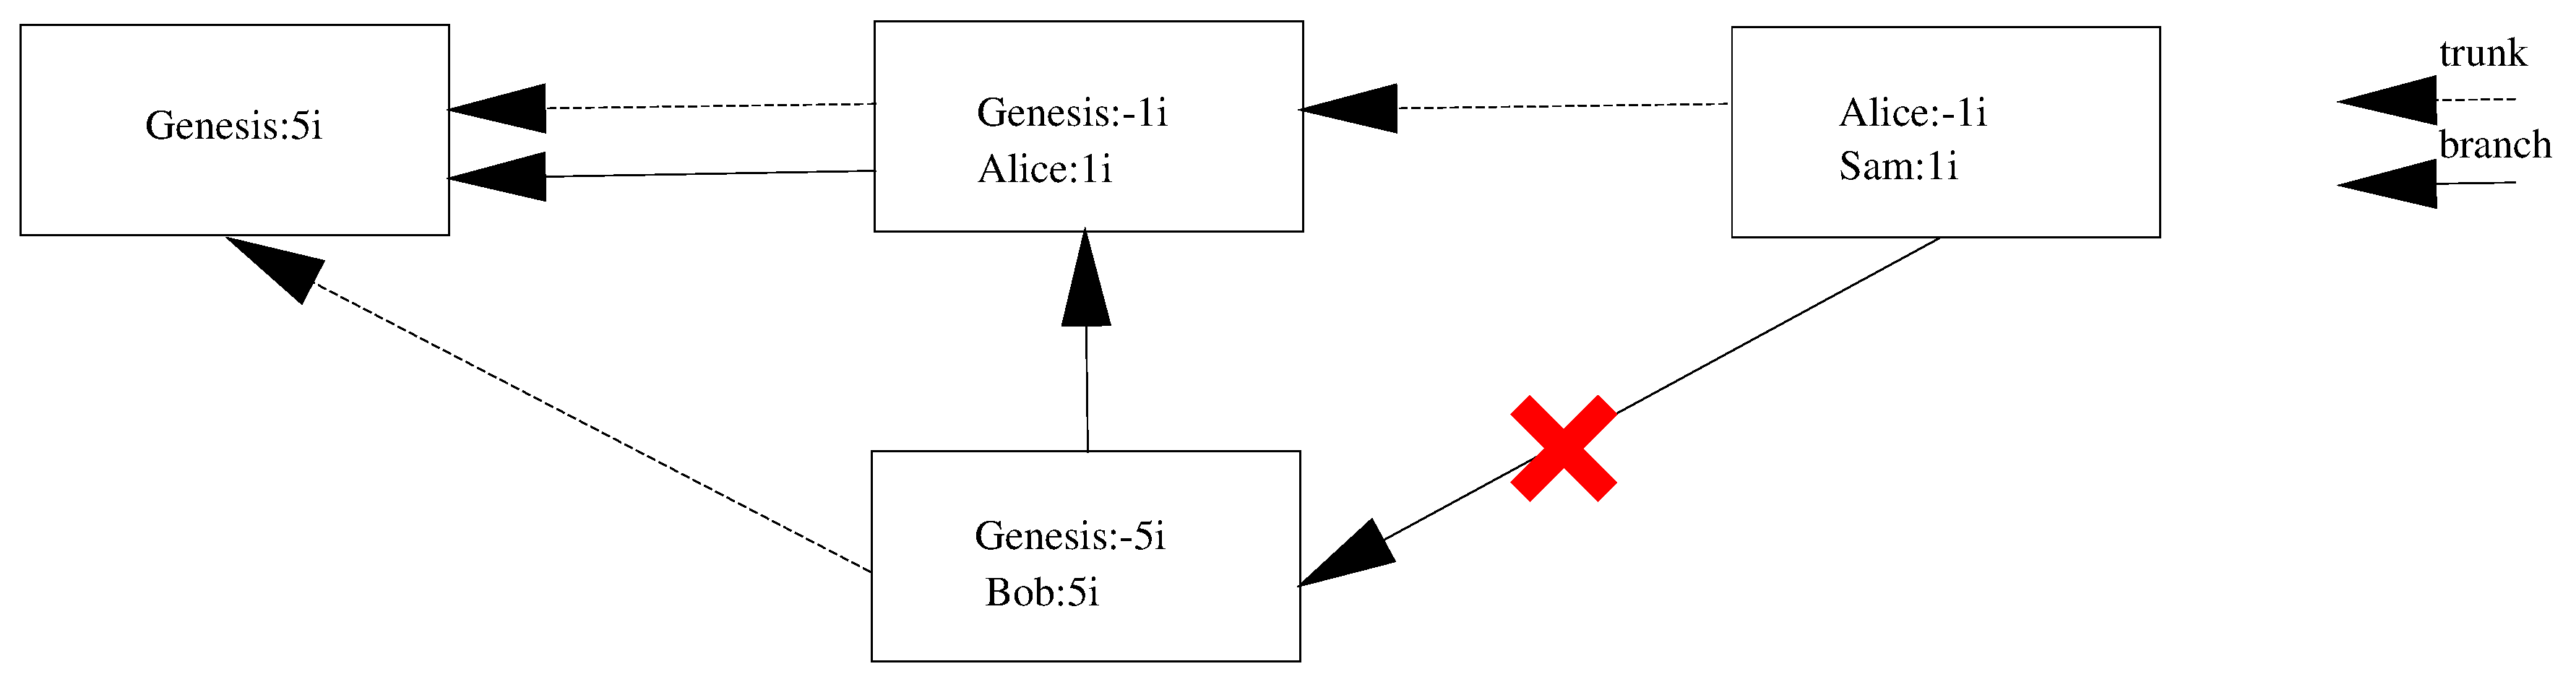
\includegraphics[width=0.35\textwidth]{figures/txn_fail.eps}
    \caption{
        An example of errornous token transfer.
     }
\label{txn_fail}
\end{center}
\end{figure}

\subsubsection{Tip Selection}
There are two basic concepts in StreamNet, one is the transaction rate $\lambda$, which indicates the number of transactions per time unit.
For convenience, we set the time unit to seconds.
The other is invisible period $h$, indicating how many time units a transaction has not been seen by other incoming blocks after attachment.
Because of $h$, the transaction rate $\lambda$ has an important influence on the shape of StreamNet.
For example, in Figure~\ref{slow_txn}, when the transaction rate is slow, StreamNet is more like a chain.
In the case of high throughput transaction in Figure~\ref{fast_txn}, the shape of StreamNet is a star.

\begin{figure}[!ht]
\begin{center}
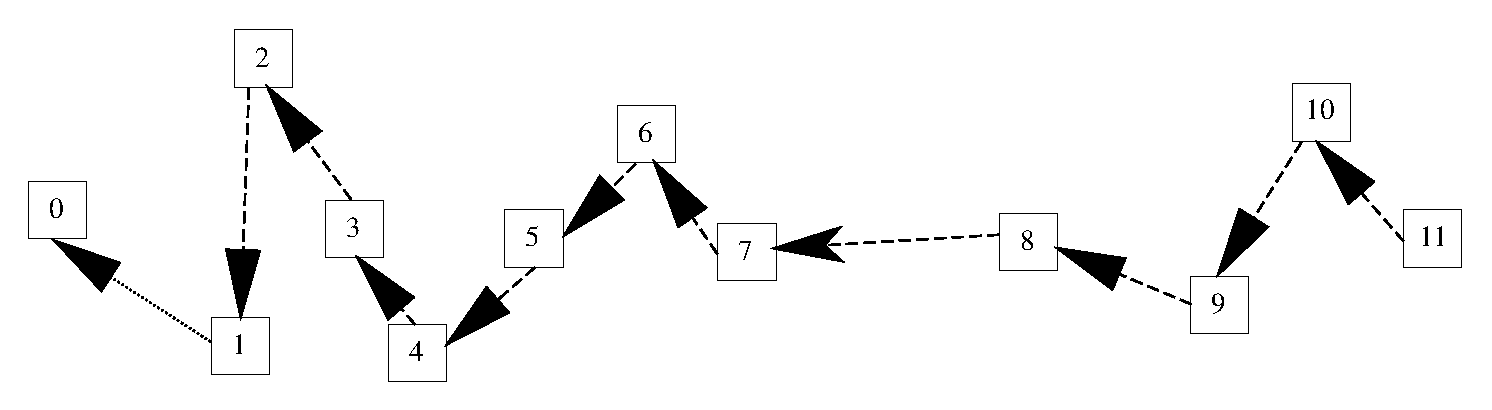
\includegraphics[width=0.35\textwidth]{figures/slow_txn.eps}
    \caption{
        The shape of StreamNet when the txn rate is low. 
     }
\label{slow_txn}
\end{center}
\end{figure}

\begin{figure}[!ht]
\begin{center}
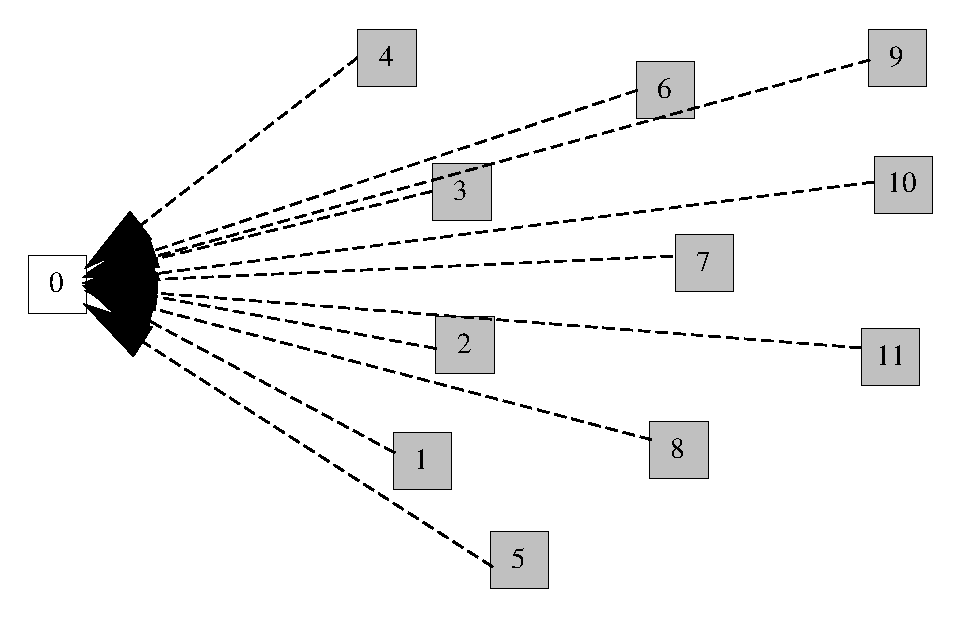
\includegraphics[width=0.35\textwidth]{figures/fast_txn.eps}
    \caption{
        The shape of StreamNet when the txn rate is high. 
     }
\label{fast_txn}
\end{center}
\end{figure}

One of simplest tip selection algorithms is the random walk with equal probability starting from Genesis, as shown in Figure~\ref{random_equal}.
Suppose Alice $\rightarrow$ Sam transaction wants to select tip, which starts from Genesis transaction.
There are two options, one is Genesis $\rightarrow$ Alice, the other is Genesis $\rightarrow$ Bob,
the probability of selecting Genesis $\rightarrow$ Alice is $\frac{1}{2}$, while Genesis $\rightarrow$ Bob is $\frac{1}{2}$. 

\begin{figure}[!ht]
\begin{center}
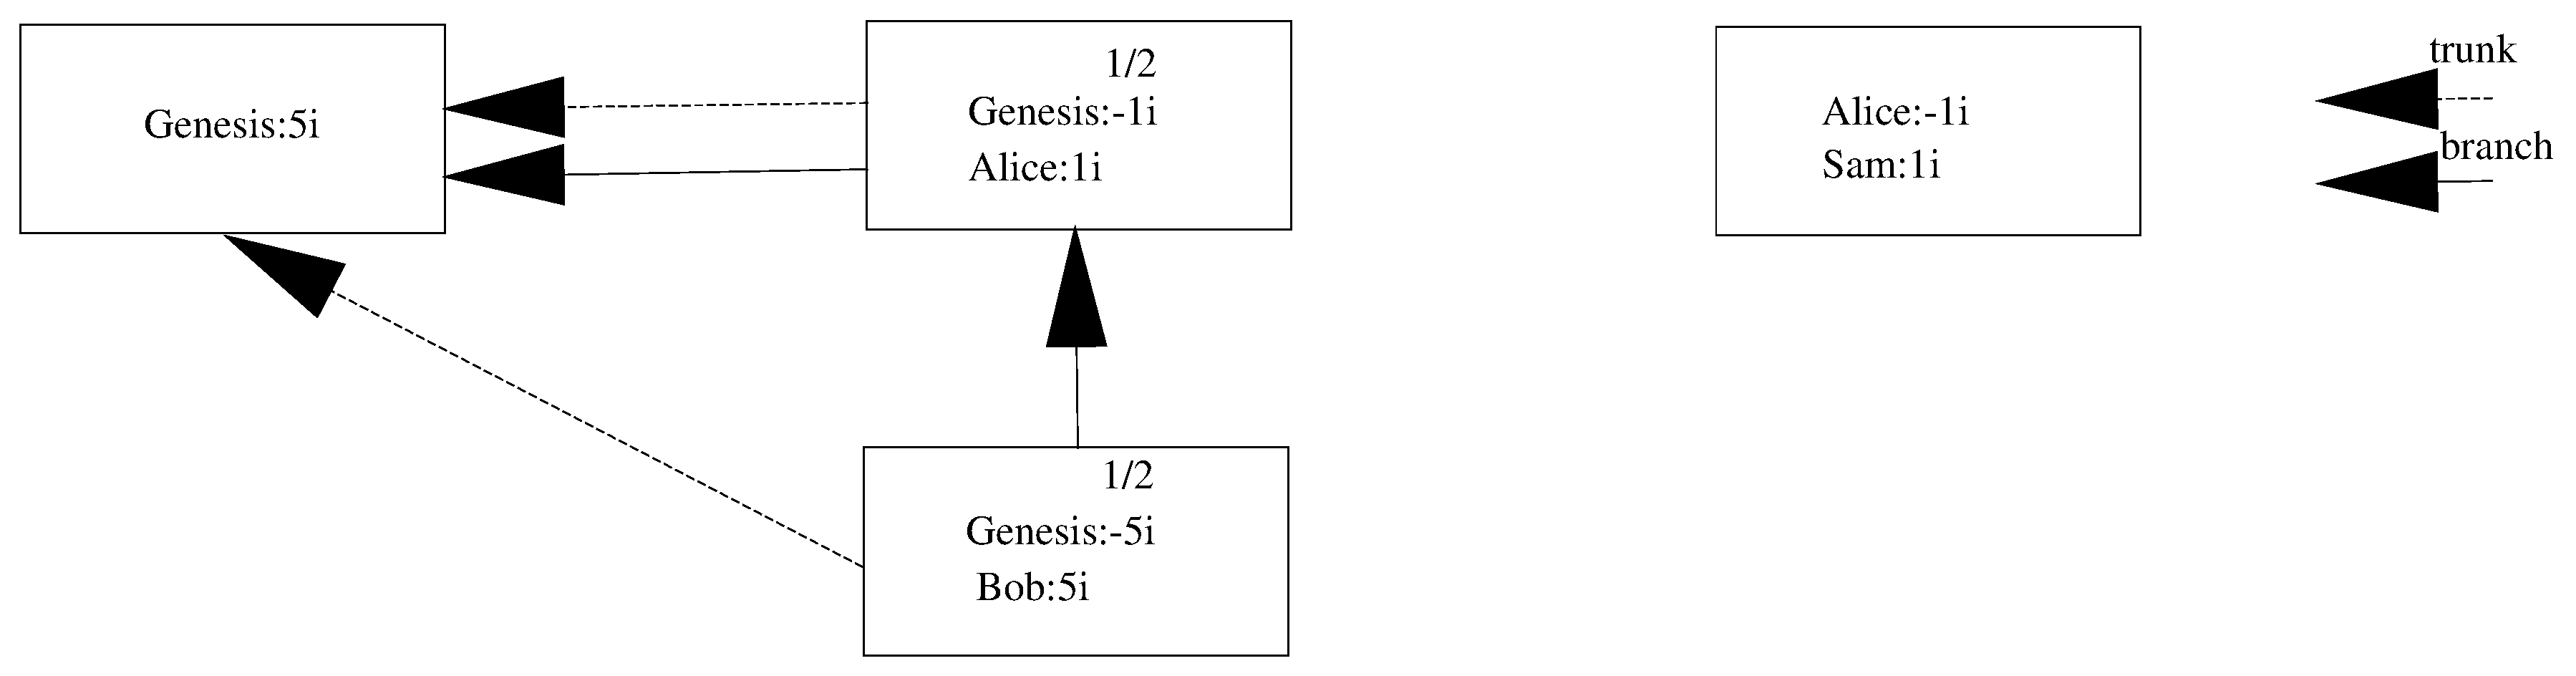
\includegraphics[width=0.35\textwidth]{figures/random_equal.eps}
    \caption{
        Random walk with equal probability.
     }
\label{random_equal}
\end{center}
\end{figure}

\begin{figure}[!ht]
\begin{center}
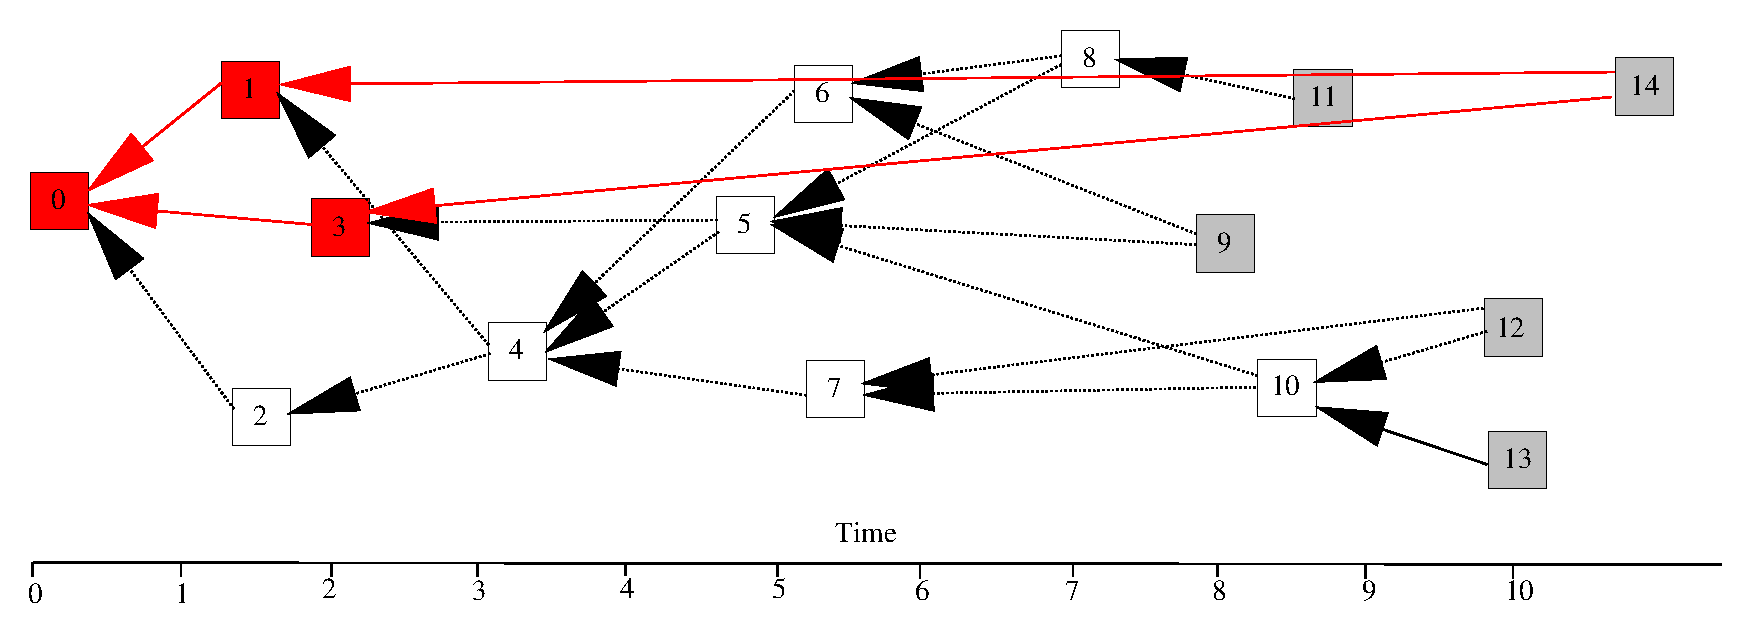
\includegraphics[width=0.35\textwidth]{figures/lazy_txn.eps}
    \caption{
        An example of lazy transaction.
     }
\label{lazy_txn}
\end{center}
\end{figure}

\begin{figure}[!ht]
\begin{center}
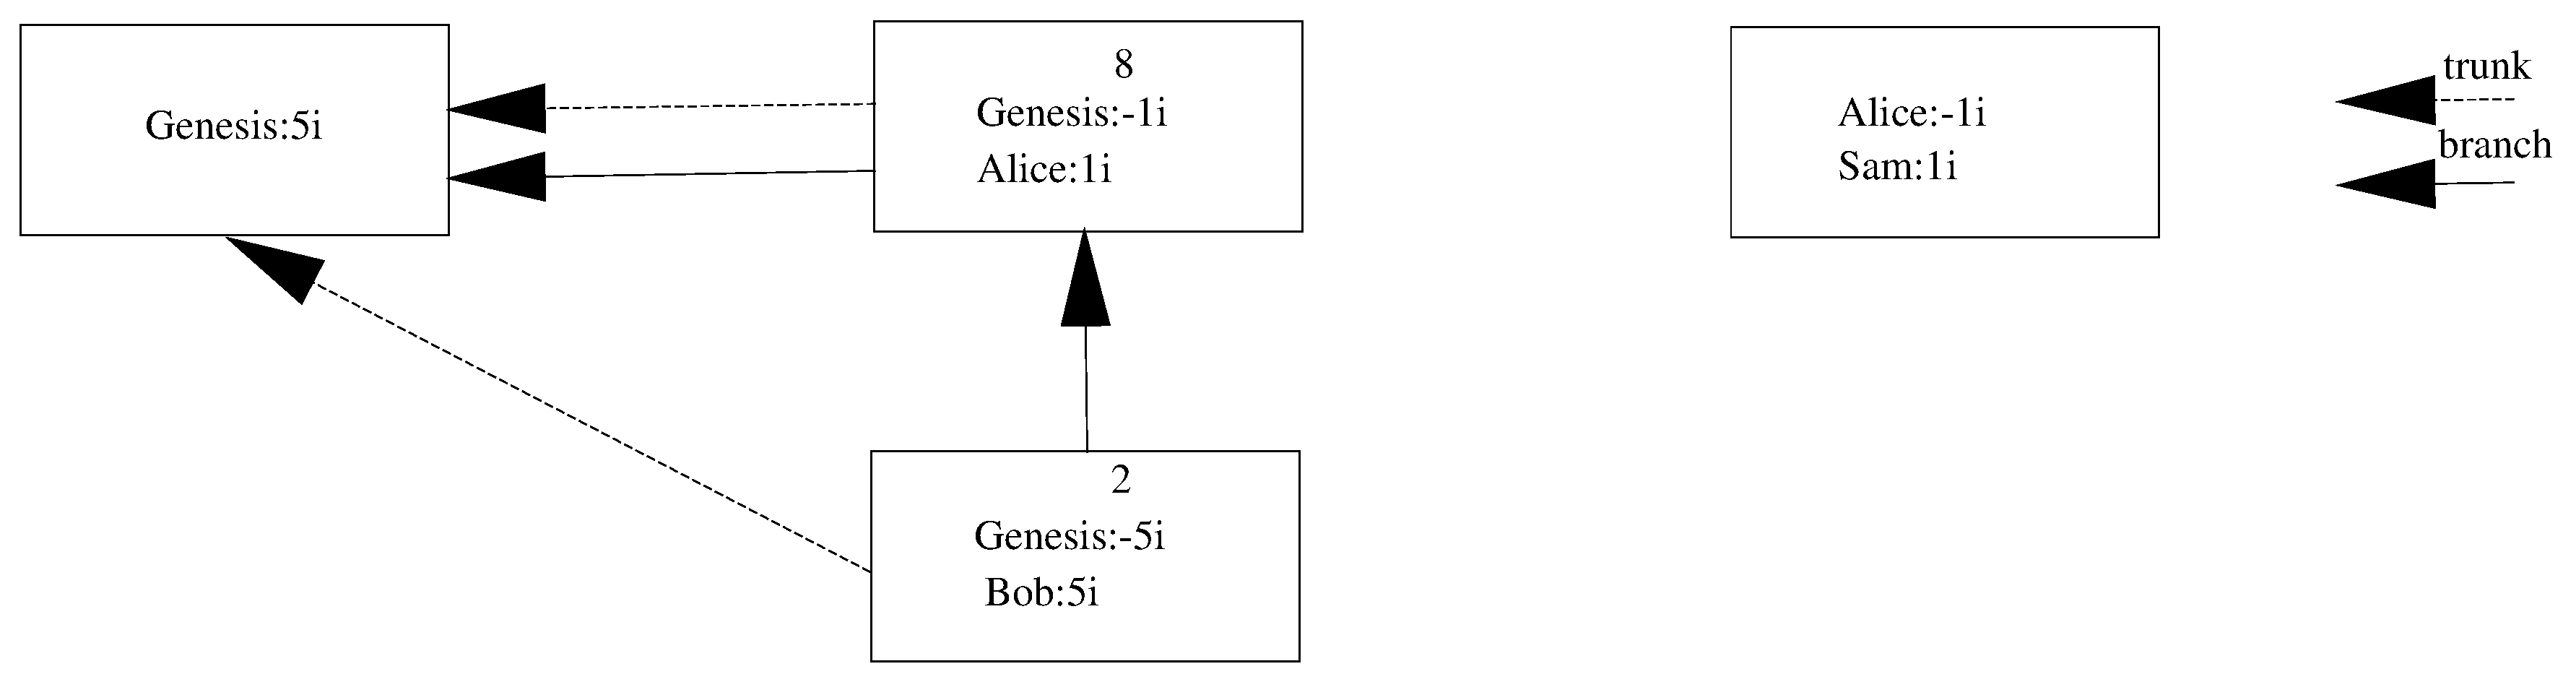
\includegraphics[width=0.35\textwidth]{figures/random_unequal.eps}
    \caption{
        Random walk with equal probability.
     }
\label{random_unequal}
\end{center}
\end{figure}

\begin{figure}[!ht]
\begin{center}
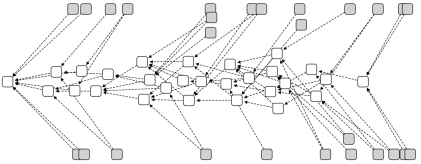
\includegraphics[width=0.35\textwidth]{figures/super_weight.png}
    \caption{
        Example of the result using super-weight algorithm.
     }
\label{super_weight}
\end{center}
\end{figure}

The problem with the simple random walk algorithm is that it produces lazy transactions.
For example, in Figure~\ref{lazy_txn}, transaction $14$ is a lazy transaction that causes new transactions to approve older transactions without being penalized.
This problem can be solved by using Monte Carlo Random Walk (MCMC).
In Figure~\ref{random_unequal}, there is a weight on both transactions, for example, Genesis $\rightarrow$ Alice is $8$, and Genesis $\rightarrow$ Bob is $2$,
then the probability of selecting Genesis $\rightarrow$ Alice is $\frac{8}{10}$,
and Genesis $\rightarrow$ Bob is $\frac{2}{10}$. 
The weight is determined by how many transactions have directly or indirectly approved the transaction.
The more approved transactions, the greater the weight.
If only weights are used then it is a super-weight algorithm, meaning that large-weight transactions are always preferred.
The problem with this algorithm is that there are many transactions that can never be confirmed.
Figure~\ref{super_weight} shows the results of a super-weighted algorithm. 
If purely using probability weighting, then it is a
super-probability algorithm. The trade-off between the two is represented by a $\alpha$, and it can be considered that the
larger the $\alpha$ is, the smaller the randomness is.
The method of specifically using $\alpha$ to calculate the jump probability is expressed in the formula (1).
Which represents the weight of the trading node.Where $P_{xy}$ represents the probability of jumping from $x$ to $y$. $H_{y}$ represents the weight of the trading node $y$.

\begin{equation}
\label{simple_equation}
P_{xy} = \frac{e^{\alpha H_{y}}}{\Sigma_{z:z \rightarrow x}e^{\alpha H_{z}}}
\end{equation}

\subsubsection{Transaction Consensus in the Gossip network}

\begin{figure*}[ht]
\begin{center}
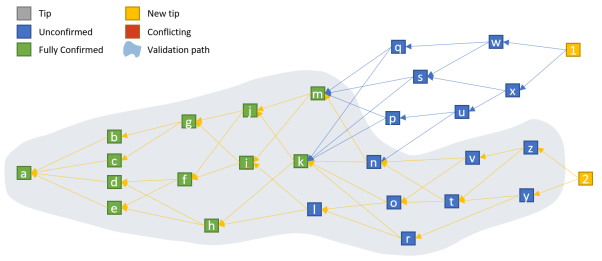
\includegraphics[width=0.65\textwidth]{figures/full_confirmation.png}
    \caption{
        Example of fully confirmed transactions.
     }
\label{full_confirmation}
\end{center}
\end{figure*}

There are currently three ways to confirm a transaction in StreamNet:
\begin{itemize}
\item The first way is that the common nodes covered by all the previous tips are considered to be fully confirmed; for example, in Figure~\ref{full_confirmation}, 
    the nodes referenced or indirectly referenced by tip1 are blue and yellow line covered transactions, 
    while the tip2 reference Or the indirectly referenced node is a yellow line covered transaction.
    If there are only 1, 2 tips in StreamNet, then the green node is a fully confirmed transaction, while the green node is an unconfirmed transaction.
\item The second way is that the system sends a Coordinator tip every 1 minute.
    This tip is called milestone and is attached to StreamNet.
    All transactions referenced by this Coordinator tip are confirmed.
\item The third way is to use Monte Carlo Random Walk (MCMC). 
    Call N times to select a tip using the tip selection algorithm.
    If a block is referenced by this tip, its credibility is increased by 1.
    After M selections have been cited M times, then the credibility is M / N.
\end{itemize}



\section{StreamNet main algorithm}

\subsection{Storage}

\subsection{UTXO and Hash Functions}
\subsubsection{Metrics for Pivotal Chain Selection}
In Phantom \cite{sompolinskyphantom} and Conflux \cite{li2018scaling}, the $GHOST$ rule \cite{sompolinsky2015secure} is applied for selecting the pivotal chain.
Here we introduce a new metric with Katz centrality \cite{katz1953new} as the weighting criteria. 
In StreamNet, we use an Adjacency Matrix to represent the direct link relationship between blocks, which is represented by $A$,
and a second-order link matrix $A^2_{ij}$ (representing the number of nodes that jump from node $i$ to node $j$ by two steps).
Similarly, we represent $k$-order adjacency matrix $A^k$.
Then the importance vector of each node can be calculated by formula (2). 
Where $\alpha$ is vector which measures the vertex importance, which $I$ is an identity matrix of all ones.
Because the transactions in StreamNet are constantly entering the network, 
if recalculate the Katz centrality every time a pivotal chain computed, 
then the complexity will be intolerable. 
So a streaming computing framework is needed. 
To dynamically update the Katz centrality based on the newly added nodes, 
we use an incremental algorithm to deal with the streaming graph calculation \cite{nathan2018incrementally}.

\begin{equation}
\label{simple_equation}
\sum_{k=1}^{max} \alpha^{k-1}A^{k}=A(I-\alpha A)^{-1}
\end{equation}

\subsection{DAG total ordering algorithm}
At any time, the local state of a user in the Conflux protocal is a graph $G = <B,g,P,E>$. $B$ is the set of blocks in $G$. $g \in G$ is the genesis block. $P$ is a function that maps a block $b$ to its parent block $P(b)$. Specially, $P(g) = \perp$. $E$ is the set of directly reference edges and parent edges in this graph. $e = <b,b^'> \in E$ is an edge from the block $b$ to the block $b^'$, which denotes that $b'$ happens before $b$. Note that there is always a parent edge from a block to its parent block (i.e., $\forall b \in B$, $b, P(b)> \in E$). All nodes in the Conflux protocal share a predefined deterministic hash function Hash that maps each block in $B$ to a unique integer id . It satisfies that $\forall {b} \neq {b'}$, Hash($b$) $\neq$ Hash($b'$).

We next define several utility functions and notatons. GetGenesis() returns the Genesis block. Past() returns the set of blocks that are generated before a given block(but include the block itself). BuildSubGraph() returns the sub graph by removing blocks and edges except the certain blocks.  In addition, a map called parentGragh is defined, key presents a block and value is the set of blocks that the block approves. Conversely, parentRevGraph construts a relationship between the block and its approvee block. Score presents the weight of blocks, each block achieves a score when attaching to the graph. 

$Pivot Chain Selection$: Figure x presents our pivot chain selection algorithm(i.e., the definition of Pivot()). Given a DAG state $G$, Pivot($G$,$g$) returns the last block in the pivot chain starting from the genesis block $g$. The algorithm recursively advances to the child block whoes corresponding subtree has the largest number of blocks. When there are multiple child blocks with the same number, the algorithm selects the child block with the largest score. The algorithm terminates until it reaches a tip. block whoes corresponding subtree has the largest number of blocks. When there are multiple child blocks with the same number, the algorithm selects the child block with the largest score. The algorithm terminates until it reaches a tip. block whoes corresponding subtree has the largest number of blocks. When there are multiple child blocks with the same number, the algorithm selects the child block with the largest score. The algorithm terminates until it reaches a tip. The algorithm is as Algorithm~\ref{algo:getPivot} shows.

\IncMargin{1em}
\begin{algorithm}
\SetKwData{Left}{left}\SetKwData{This}{this}\SetKwData{Up}{up}
\SetKwFunction{Union}{Union}\SetKwFunction{FindCompress}{FindCompress}
\SetKwInOut{Input}{input}\SetKwInOut{Output}{output}

\KwIn{ The local state $G$ = $<B,g,P,E>$  and a starting block $b \in B$ }
\KwOut{ The last block in the pivot chain for the subtree of $b$ in $G$ }

\Do { Child(G,b) != 0} {
  $b'$ $\longleftarrow$ Child($G,b$)  \;
  $tmpMaxScore$ $\longleftarrow$ -1 \;
  $tmpBlock$ $\longleftarrow$ $\perp$ \;
  \Do { $b'$ $\neq$ 0 } {
    $score$ $\longleftarrow$ Score($G, b'$) \;
    \If { $score$ $>$ $tmpMaxScore$ $||$ ($score$ = $tmpMaxScore$ \text{and Hash($b'$ ) $<$ Hash($tmpBlock$)}} {
      $tmpMaxScore$ $\longleftarrow$ $score$ \;
      $tmpBlock$ $\longleftarrow$ $b'$ \; 
    }
  }
  $b$ $\longleftarrow$ $tmpBlock$ \;
}

\Return{$tmpBlock$} \;

\caption{{\sc pivot block($G$, $b$).}}
\label{algo:getPivot}
\end{algorithm}
\DecMargin{1em}



$Total Order$: Figure x defines ConfluxOrder(), which corresponds to our block ordering algorithm. Given the local state $G$ and a block $a$ in the pivot chain, ConfluxOrder($G$,$a$) returns the ordered list of all blocks that appear in or before the epoch of $a$. Using ConfluxOrder(), the total order of a local state $G$ is defined as TotalOrder($G$) in Figure x. The algorithm in Figure x first recursively orders all blocks in previous epochs(i.e., the epoch of $P(a)$ and before). It then computes all blocks in the epoch of $a$ as $B_\Delta$. It topologically sorts all blocks in $B_\Delta$ and appends it into the result list. The algorithm uses the unique hash to break ties. The algorithm is as Algorithm~\ref{algo:conflux_order} shows;

\IncMargin{1em}
\begin{algorithm}
\SetKwData{Left}{left}\SetKwData{This}{this}\SetKwData{Up}{up}
\SetKwFunction{Union}{Union}\SetKwFunction{FindCompress}{FindCompress}
\SetKwInOut{Input}{input}\SetKwInOut{Output}{output}

\KwIn{ The local state $G$ = $<B,g,P,E>$  and a tip block $b \in B$ }
\KwOut{ The block list of total top order starting from Genesis block to the giving block $b$ in $G$ }

$L = \perp$

\Do { $b$ != $g$} {
  $p$ $\gets$ Parent($G,b$)  \;
  $B_\Delta$ $\gets$ Past($G$,$b$) - Past($G$,$p$) \;
  \Do { $B_\Delta$ $\neq$ 0 } {
      $G'$ $\gets SubGraph(B_\Delta) $ \;
    $B'_\Delta$ $\gets$ \{x $||$ Before($G'$,$x$) = 0\} \;
    \text{Sort all blocks in $B'_\Delta$ in order as $b'_1,b'_2,...,b'_k$} \\
      \text{such that $\forall$1$\leq i \leq j \leq k$, Hash($b'_i$) $\leq$ Hash($b'_j$)} \;  
    $L$ $\gets$ $L + b'_1 + b'_2 + ... + b'_k$ \;
    $B_\Delta$ $\gets$ $B_\Delta$ - $B'_\Delta$ \;
  }
  $b$ = $p$ \;
}


\Return{$L$} \;

\caption{{\sc StreamNetOrder($G$, $b$).}}
\label{algo:conflux_order}
\end{algorithm}
\DecMargin{1em}


\begin{figure}
\begin{equation*}
%  Chain(G,b) &= 
%  \begin{cases}
%    g                 & b = g\\
%    Chain(G,P(b))     & \text{otherwise}
%  \end{cases}\\
%  Child(G,b) &= \{ b'| P(b') = b \}\\
%  Sibling(G,b) &= Child(G,P(b))\\
%  Substree(G,b) &= (U_{i\in Child(G,b)}Substree(G,i))U\{b\}\\
%  Before(G,b) &= \{b'|b' \in B, <b,b'> \in E \}\\
%  Past(G,b) = (U_{i\in Before(G,b)}Past(G,i))U\{b\}\\
%  TotalOrder(G) &= ConfluxOrder(G,Pivot(G,g))
  \text{ TODO method list }
\end{equation*}
\label{totalFormulas}
\caption{ The Definitions of Chain(),Child(),Sibling(),Subtree(),Before(),Past() and TotalOrder(). }
\end{figure}
% TODO how to layout the formulas above ?

\subsection{Tip Selection Algorithm with Configurable Local Modifiers}

In $StreamNet$, when one new block wants to be attached to the main network, it should find a parent block and a reference block. We call this procedure the tip selection method. 
The parent block is found by calling the total ordering algorithm and the reference block is found by calling the $MCMC$ from the entry point. The algorithm is as Algorithm~\ref{algo:tip_sel} shows.

\IncMargin{1em}
\begin{algorithm}
\SetKwData{Left}{left}\SetKwData{This}{this}\SetKwData{Up}{up}
\SetKwFunction{Union}{Union}\SetKwFunction{FindCompress}{FindCompress}
\SetKwInOut{Input}{input}\SetKwInOut{Output}{output}

\KwIn{ Graph $G$, Block $B$, score $S$, random walker $W$, and depth $d$ }
\KwOut{Parent tip $T_p$ and reference tip $T_r$ }

$totalOrderChain$ = totalOrder($G$, $B$) \;
$T_p$ = $totalOrderChain$.last() \;
$entryPoint$ = $totalOrderChain$.at($d$) \; 

\Do {localModifier($T_r$) != $false$} {
    $T_r$ = $W$.Walk($G$, $S$, $entryPoint$) \;
}
%} 

\Return{$T_p$, $T_r$} \;

\caption{{\sc Tip selection tipSel($G$, $B$, $S$, $W$, $d$).}}
\label{algo:tip_sel}
\end{algorithm}
\DecMargin{1em}


\subsubsection{Entrypoint selection}
When performing tip selection, an entry point is neccessary, and in $IOTA$ mainet, it will not start from the genesis transaction,
but will simply start from a coordinator ($COO$) as the entry point.
This will leads to a centralization problem. 
So one of the most important question we considered when designing StreamNet was how to remove $COO$ and achieve a truly decentralized $DAG$. 
So we need a consensus authoritative transaction as a entrypoint rather than a coordinator mandated by a centralized node.
It should be noted that we do not need to find the transaction with the largest Katz centrality score in the whole network,
because this transaction is always the Genesis transaction.
So we specify a depth and find the block with this depth on pivotal chain.

\subsubsection{Local Modifier Considering Edge Information}

\begin{figure}[!ht]
\begin{center}
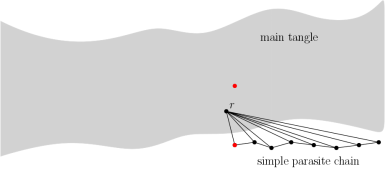
\includegraphics[width=0.45\textwidth]{figures/spc.png}
    \caption{
        An example of simple parasite chain attack, a series of cheat transaction will refer one specific double spent transaction, 
        when the $SPC$ grows to a certain amount, the double spent will be successful, the two red node in the figure respents the 
        conflict transactions.
     }
\label{spc}
\end{center}
\end{figure}


Because the attacker can attack the main network (Main StreamNet) in different forms,
a typical scenario in which we consider the double-spending problem is the Simple Parasite Chain attack.
A simple side chain is shown in Figure~\ref{spc}. 
In \cite{iota_proof}, the author proposed to use local modifier to solve the attack. And in our tip selection algorithm, 
the local modifier is used for filtering malformed tips and the strategy is configurrable. 
Here we discuss one of the local modifier with edge information.
The framework of this algorithm is consistent with the framework of the weight update algorithm in the existing DAG.
The difference is that when making a set join between two approve transactions, a weighted set join is performed, and the weight is determined by edges. 
And the information of the edge is mainly determined by time information. 
For example, in Figure~\ref{edge_info}, assume that each edge is assigned a weight $w1$ to $w12$, 
because transaction $5$ is approved by transactions $6$, $7$, $8$, as a result its weight is $(w1+w2+w3+w6+w1 \cdot w6)$.

The reason for the adding of edge information is that the attacker often sends out a large number of transactions 
within a short period of time to achieve the purpose of rapidly growing the side chain. 
If edge information is used to rescale the weight, the effects of these attacks are attenuated. 
On the contrary, becasue the issuing rate of non-attack type transaction is similar to the speed of the whole network,
and its weight update is similar to the result of the original algorithm.

\begin{figure}[!ht]
\begin{center}
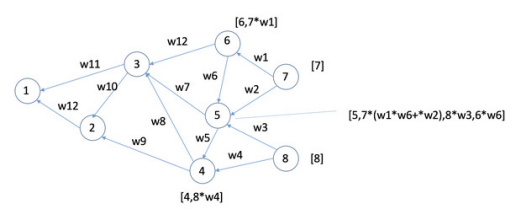
\includegraphics[width=0.55\textwidth]{figures/edge_info.png}
    \caption{
        Weight calculation based on edge information.
     }
\label{edge_info}
\end{center}
\end{figure}


\section{Experimental Results}

\subsection{Implementation}
We have implemented the StreamNet based on the IOTA JAVA reference code (IRI) v1.5.5 \cite{IOTACode}.

\begin{itemize}
    \item The features we have adopted from the IRI are: 
    \begin{itemize}
        \item The block header format;
        \item Gossip network;
        \item Trasnaction bundle, because of the existence of the bundle hash feature, StreamNet can support both the single transaction for a block and batched transactions as a bundle. 
        \item Sponge hash functions which is claimed to be quantum immune, in our experiment, the POW hardness is set to 8 which is the same as the testnet for IOTA.
    \end{itemize}

    \item The features we have abandoned from the IRI are:
    \begin{itemize}
        \item The iota's transaction logic inlcuding the ledger part;
        \item The milestone issued by coordinators. 
    \end{itemize}

    \item The features we have modified based on the IRI is: 
    \begin{itemize}
        \item The tip selection method based on MCMC, since the tip selection on IRI has to find a milestone to start searching, we replace this with a block in the pivotal chain instead.
    \end{itemize}


    \item The features we have added into the StreamNet are: 
    \begin{itemize}
        \item The consensus algorithms; 
        \item The UTXO logic which is stored in the signature part of the block header. 
        \item In IOTA's implementation, the blocks are stored in the RocksDB \cite{RocksDB} as the persistence layer, which makes it inefficient to infer the relationships between blocks and calculate graph features. In our implementation, we introduced an in-memory layer to store the relationships between blocks, such that the tip selection and total ordering algorithm will be accelerated. 
    \end{itemize}
\end{itemize}

\subsection {Environment Set Up}

We have used the tencent cloud services, for each virtual machine, it includes a two core Intel(R) Xeon(R) CPU E5-26xx v4, with 3 Gb of memory size and 118Gb of disk size. The JAVA version is 1.8, we have deployed our service using docker and the docker version is 18.02.0-ce.   

We have 7 machines set up, and they are connected into a gossip network in a cycle or in a clique. the requests will be distributed to these machines evenly.
As for the data, we have created 10,000 accounts, with the genesis account having 100,000,000,000 tokens in the coinbase block.
And we have issued 1,000,000 transactions in the network with 100 threads.
Jmeter is utilized as the driver to issue the transactions and nginx is used to evenly distribute the requests to different nodes.

\subsection {Results and Discussions}

\subsubsection {Single transaction test}
By default, each block in StreamNet will only support one transaction. And the performance on this configuration is as Figure~\ref{single_txn} shows.

\begin{figure}[!ht]
\begin{center}
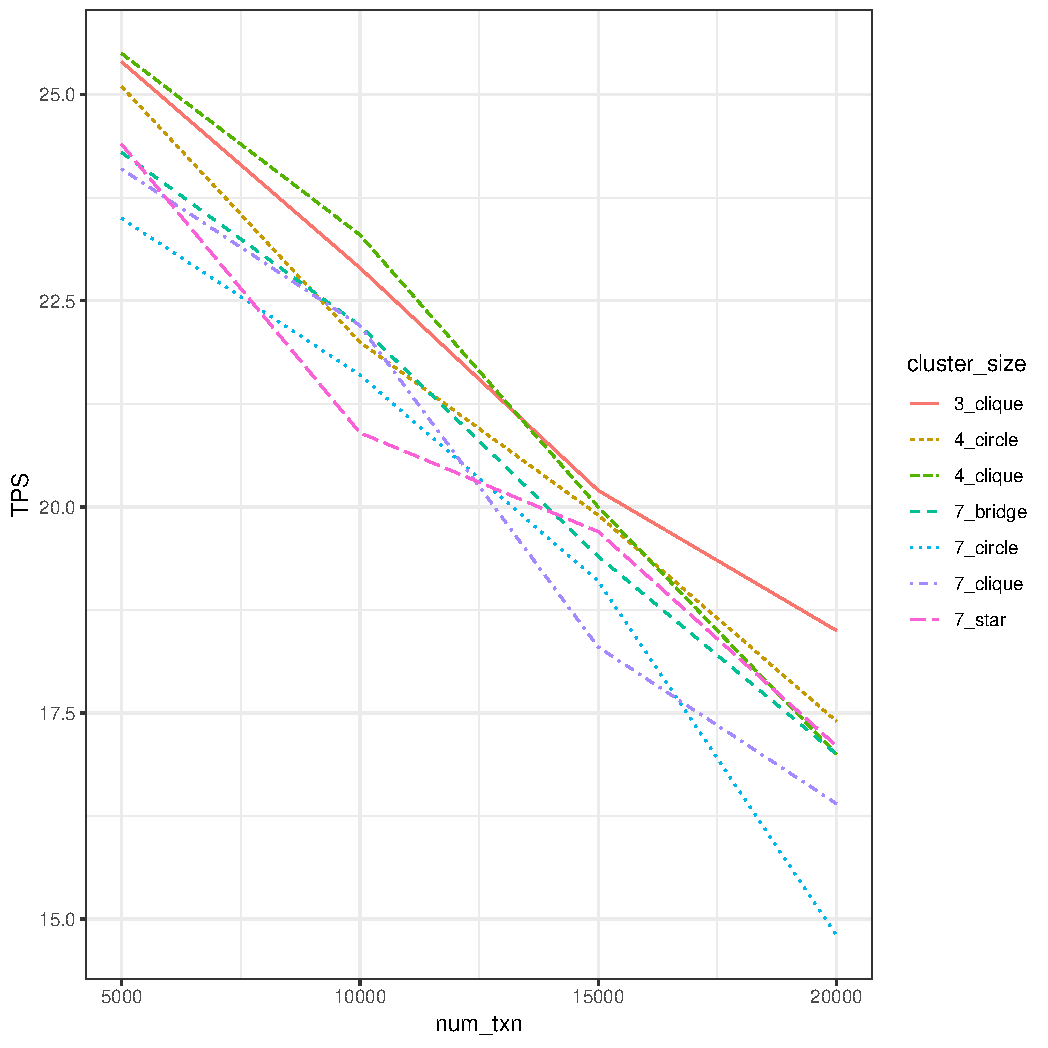
\includegraphics[width=0.45\textwidth]{figures/single_txn.pdf}
    \caption{
        Experimental results for single transaction.
     }
\label{single_txn}
\end{center}
\end{figure}



\subsubsection {Bundle transaction test}

By default, each block in StreamNet will only support one transaction. And the performance on this configuration is as Figure~\ref{single_txn} shows.

\begin{figure}[!ht]
\begin{center}
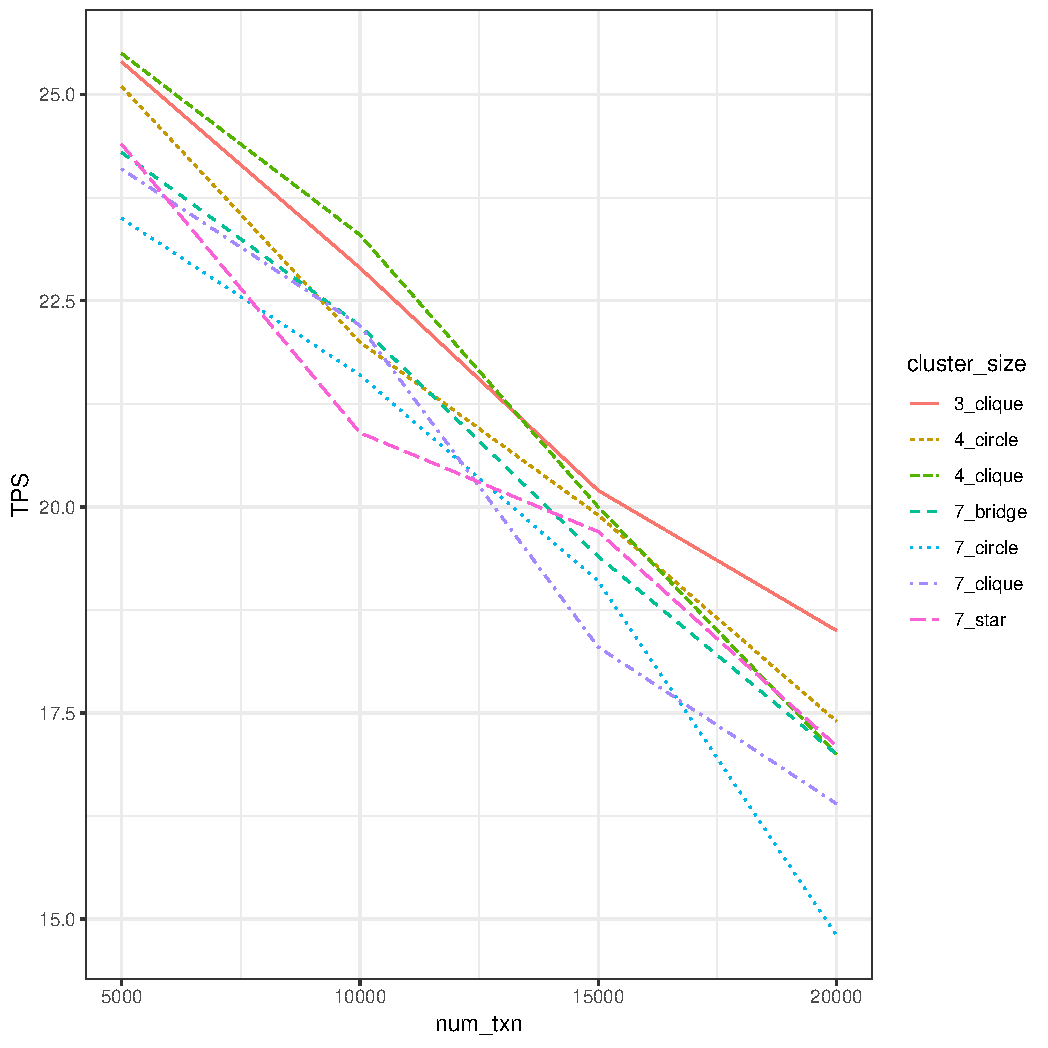
\includegraphics[width=0.45\textwidth]{figures/single_txn.pdf}
    \caption{
        Experimental results for single transaction.
     }
\label{single_txn}
\end{center}
\end{figure}



\section{Conclusion}
In this paper, we proposed a way to compute how to grow the blocks in the growing DAG based blockchain systems. 
And how to maintain the total order as the DAG structure is dynamically turning larger.
We referred one of the earliest DAG implementation IRI to conduct our own experiments on clusters of different size and topology. 
Despite the network inefficiency in the IRI implementation, 
our method is proven to be able to tolerate the increasing complexity of the graph computation problems involved. 
This is due to the streaming graph computing techniques we have introduced in this paper.


\bibliographystyle{ACM-Reference-Format}
\bibliography{StreamNet}


\end{document}
